\chapter{Subdivision Plugin}

Die Hauptfunktionalität des Programms SubVis wird ebenfalls in einem Plugin bereitgestellt. 
Dieses erlaubt die Anwendung verschiedener Unterteilungsalgorithmen und das Rendering deren Limes-Flächen.

\begin{figure}
  \centering
  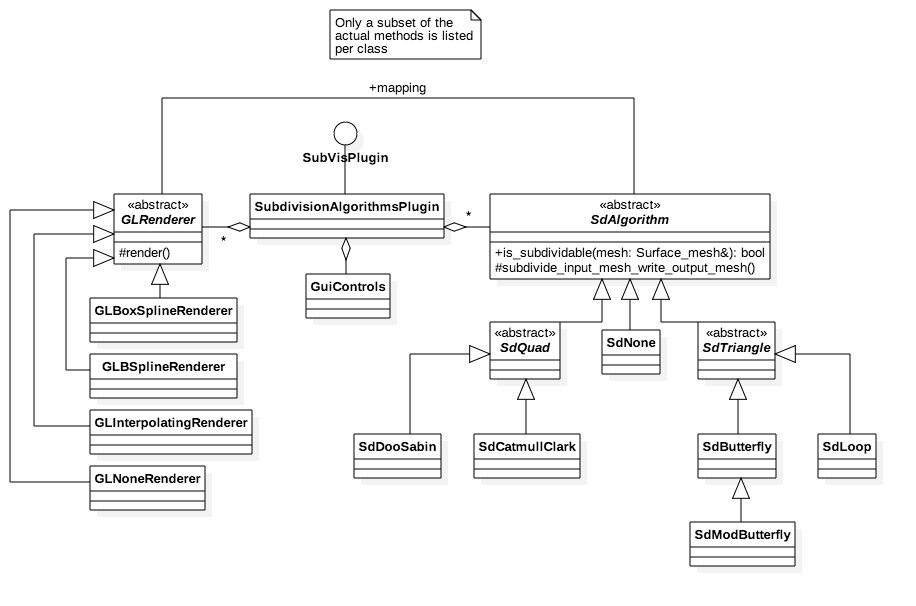
\includegraphics[width=\textwidth]{content/media/subvis_architektur_plugin_subdivision.png}
  \caption{Architektur des Subdivision-Plugins}
  \label{fig:subvis_architektur_plugin_subdivision}
\end{figure}

\autoref{fig:subvis_architektur_plugin_subdivision} gibt einen Überblick über die Architektur.
Die Hauptklasse ist \emph{SubdivisionAlgorithmsPlugin} welche auch die SubVisPlugin Schnittstelle implementiert.
Die GUI, das Rendering und die Algorithmen wurden in jeweils eigene Klassen ausgelagert.

\section{GUI}

\begin{figure}
  \centering
  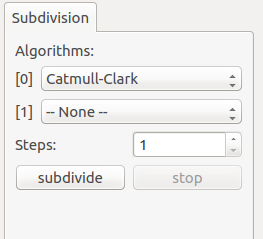
\includegraphics[width=0.3\textwidth]{content/media/subvis_plugin.png}
  \caption{GUI-Elemente des Plugins}
  \label{fig:subivs_plugin_gui}
\end{figure}

Die GUI besteht aus zwei Auswahllisten für den Algorithmus pro Polygonnetz, einer Einstellung für die Anzahl an Unterteilungsschritten und einem Start bzw. Stop Button (siehe \autoref{fig:subivs_plugin_gui}).

\section{Rendering}

Jeder Renderer erweitert die abstrakte Klasse \emph{GLRenderer}. 
Diese ruft mittels Template-Pattern eine Methode \emph{render} ihrer Unterklasse auf, um den Rendervorgang zu starten.
Bei Veränderungen der Model-Komponente wird das Polygonnetz kopiert, damit Unterklassen das Polygonnetz verändern können.
Ziel ist es die Limesfläche des Kontrollnetzes zu rendern.
Abhängig vom angewendeten Unterteilungsalgorithmus wird die
Limesfläche unterschiedlich berechnet.

\subsection{Interpolating Renderer}
Bei dem Modified Butterfly und dem Butterfly Algorithmus handelt es sich um
interpolierende Unterteilungsalgorithmen.
Hier geht die Limesfäche durch das Kontrollnetz und es wird ein
interpolierender Renderer benötigt.
Die Kontrollpunkte werden interpoliert und die
Oberflächenbeläuchtung anhand der Vertex Normalen berechnet,
sodass die Oberfläche glatt erscheint.


\subsection{B-Spline Renderer}
Catmull-Clark und Doo-Sabin sind Unterteilungsalgorithmen auf Basis von
kubischen und quadratischen B-Splines.
Für ein Rendering kann die B-Spline Tensorproduktfläche nach Bezier gewandelt werden.
Die Kontrollpunkte können dann als Bezier Tensorproduktfläche interpretiert werden.
Aktuell ist an dieser Stelle noch der \emph{Interpolating Renderer} implementiert.

//TODO Tobi

\subsection{Box-Spline Renderer}
Der Unterteilungsalgorithmus Loop basiert auf Box-Splines.
Die Fläche kann zum Rendern in ein Bezier-Dreiecksnetz gewandelt werden.
Aktuell ist an dieser Stelle noch der \emph{Interpolating Renderer} implementiert.

//TODO Tobi

\subsection{None Renderer}
Der None Renderer ist eine Dummy Implementierung für den Fall,
dass kein Unterteilungsalgorithmus ausgewählt ist.
Dann wird nichts dargestellt.

\section{Algorithmen}

Die Algorithmen werden über die abstrakte Klasse \emph{SdAlgorithm} zusammengefasst. 
Diese ermöglicht es, der GUI abzufragen, ob ein bestimmtes Polygonnetz von diesem Algorithmus unterteilt werden kann oder nicht, was sich in der Auswahlmöglichkeit der GUI niederschlägt.
Außerdem implementiert die Klasse die Verwaltung der Polygonnetze und ein Thread-basiertes unterteilen. 
Somit müssen die konkreten Klassen der Algorithmen lediglich eine Methode überschreiben und sich nur auf die korrekte Implementierung fokussieren.
Es werden vor jedem Aufruf der Unterklasse die Variablen \emph{input\_mesh} und \emph{output\_mesh} entsprechend initialisiert.
Die Unterklassen müssen dann pro Aufruf von \emph{subdivide\_input\_mesh\_write\_output\_mesh} das Eingangsnetz lesen und das Ergebnis in der Variable output\_mesh speichern.

\begin{lstlisting}[style=myCppStyle, caption={Signatur der Unterteilungsfunktion}, label=lst:subdiv_threaded]
void subdivide_threaded(const Surface_mesh& mesh, 
std::function<void(std::unique_ptr<Surface_mesh>)> callback, 
const int steps = 1);
\end{lstlisting}

Das Thread-basierte Rendering ist über einen Callback-Mechanismus implementiert (vgl. \autoref{lst:subdiv_threaded}), welcher garantiert, dass die Callback-Funktion auf dem UI-Thread ausgeführt wird.
Die Funktion subdivide\_threaded ruft eine Worker-Funktion mittels QtConcurrent::run auf, welche in einer Schleife die konkrete Implementierung der Unterteilung ausführt.
Die Worker-Funktion sendet am Ende ihrer Ausführung ein Signal \emph{finished} aus.
Dieses wiederum wird von der Klasse empfangen und in einen Aufruf der Callback-Funktion umgesetzt.
Durch Verwendung des Signal-Slot Konzepts ist garantiert, dass der Slot und somit der Callback auf dem UI-Thread ausgeführt wird.
Der implementierte Callback-Mechanismus macht somit das Threading wesentlich einfacher und benötigt keine Synchronisierungsmechanismen.

Als konkreter Callback wird eine Funktion verwendet, die bei Beendigung das Ergebnis in die Model-Komponente lädt (was ein Neuzeichnen des Polygonnetzes zur Folge hat).

\subsection{Vererbungshierarchie}

\emph{SdAlgorithm} ist die Klasse, von der alle Unterteilungsalgorithmen abgeleitet werden.
Diese Klasse implementiert wie bereits beschrieben alle Basisfunktionen.
Die Algorithmen Catmull-Clark, Doo-Sabin, Loop, Butterfly und Modified Butterfly lassen sich aber
noch weiter klassifizieren und zusammenfassen.
Daher wurden die beiden Unterflassen \emph{SdQuad} und \emph{SdTriangle} eingeführt,
die von \emph{SdAlgorithm} erben.

\emph{SdQuad} vereinigt gemeinsame Funktionen von Catmull-Clark und Doo-Sabin.
Dazu gehört das Verwalten von Properties (Edge Point, Face Point \ldots) und
die Berechnung des Face Points.

\emph{SdTriangle} fasst die Unterteilungsalgorithmen für Dreiecksnetze zusammen.
Loop, Butterfly und Modified Butterfly verwenden die gleiche Face Split Funktion
und benötigen ähnlichen Properties.

Die konkreten Implementierungen der Unterteilungsalgorithmen erben schließlich
von \emph{SdQuad} oder \emph{SdTriangle}.
Durch diese Architektur kann redundanter Code vermieden werden.


\subsection{Catmull-Clark}

Die Implementierung des Unterteilungsalgorithmus ist wie in \autoref{sec:catmull}
beschrieben. \emph{SdCatmull} erbt von \emph{SdQuad}.
Der Algorithmus kann mit einem beliebigen Polygonnetz umgehen.
Die Randregeln sind vollständig umgesetzt.
\autoref{fig:sd_catmull_screenshot} zeigt einen Würfel und das Netz nach
einer Unterteilung.

\begin{figure}
  \centering
  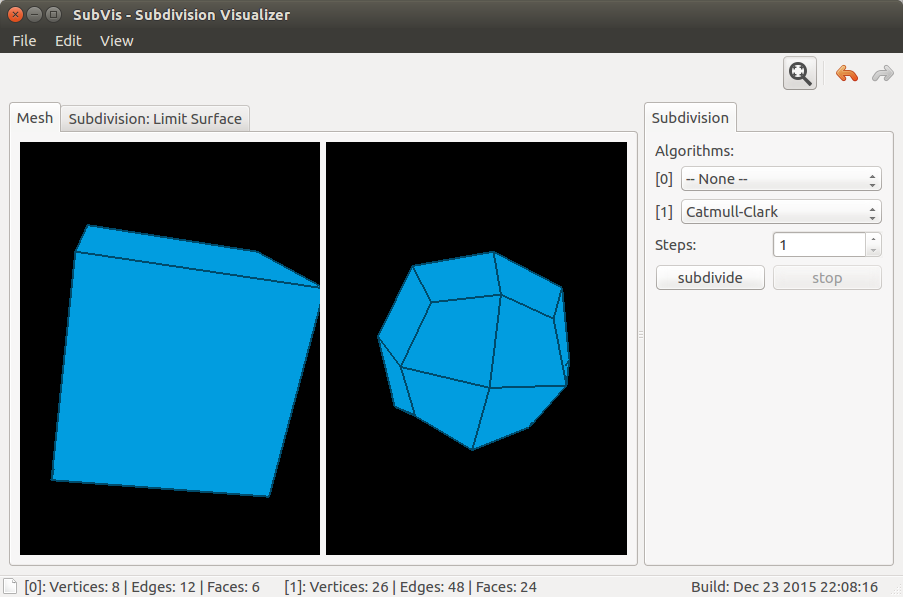
\includegraphics[width=0.7\textwidth]{content/media/sd_catmull_screenshot.png}
  \caption{Subvis - Catmull-Clark}
  \label{fig:sd_catmull_screenshot}
\end{figure}


\subsection{Doo-Sabin}

Doo-Sabin ist inklusive Randregel wie in \autoref{sec:doosabin}
gezeigt umgesetzt. Die Klasse \emph{SdDooSabin} erbt von \emph{SdQuad}.
\autoref{fig:sd_catmull_screenshot} zeigt einen Unterteilungsschritt eines Würfels.

\begin{figure}
  \centering
  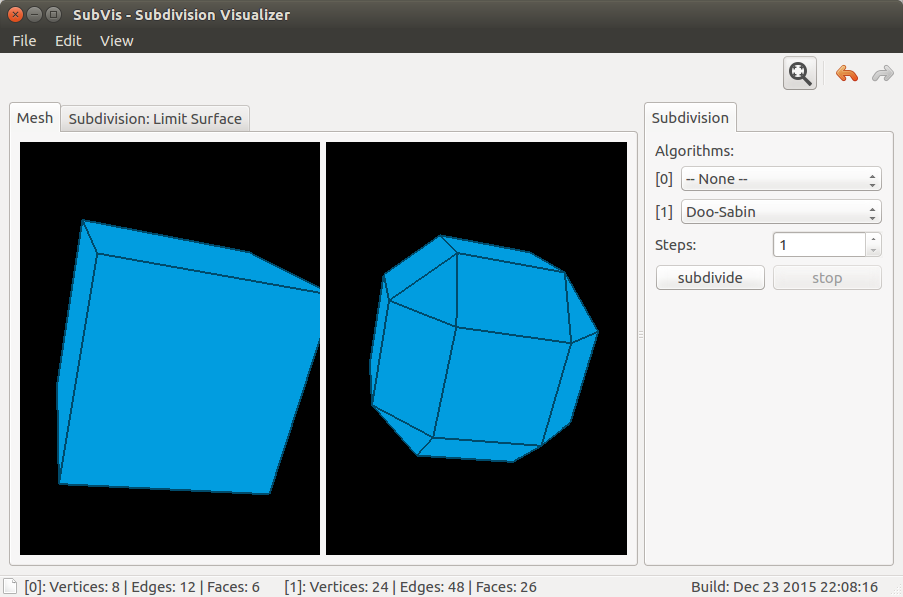
\includegraphics[width=0.7\textwidth]{content/media/sd_doosabin_screenshot.png}
  \caption{Subvis - Doo-Sabin}
  \label{fig:sd_doosabin_screenshot}
\end{figure}

\subsection{Loop}

Loop ist in der Klasse \emph{SdLoop} implementiert und erbt von \emph{SdTrianlge}.
Die Implementierung erfolgt wie in \autoref{sec:loop} beschrieben
und unterstützt die gezeigten Randregeln.
\autoref{fig:sd_loop_screenshot} zeigt die Unterteilung eines Icosahedrons.

\begin{figure}
  \centering
  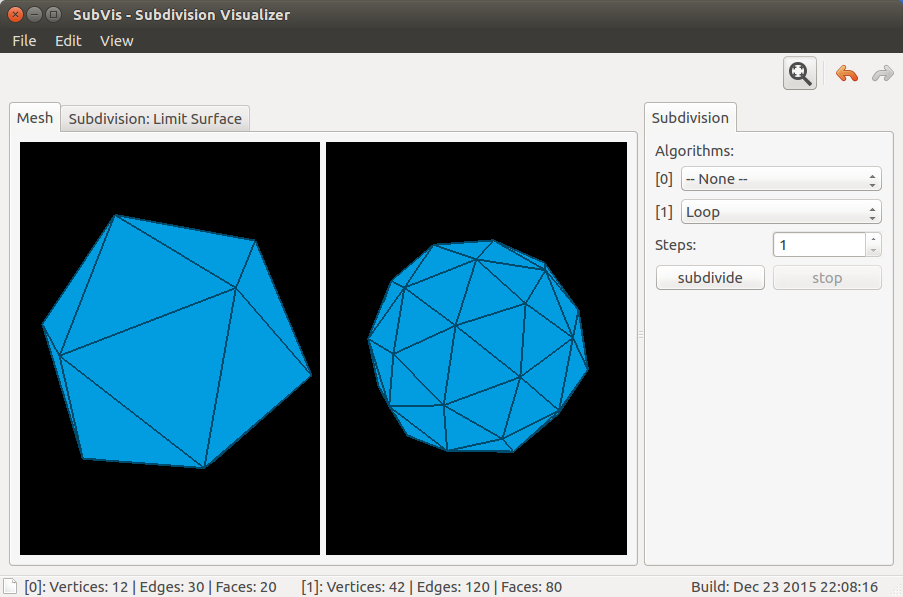
\includegraphics[width=0.7\textwidth]{content/media/sd_loop_screenshot.png}
  \caption{Subvis - Loop}
  \label{fig:sd_loop_screenshot}
\end{figure}

\subsection{Butterfly}

Der Butterfly Algorithmus ist nach \autoref{sec:butterfly}
in der Klasse \emph{SdButterfly} implementiert.
\emph{SdButterfly} erbt von \emph{SdTrianlge}.
\autoref{fig:sd_butterfly_screenshot} zeigt einen Unterteilungsschritt.

\begin{figure}
  \centering
  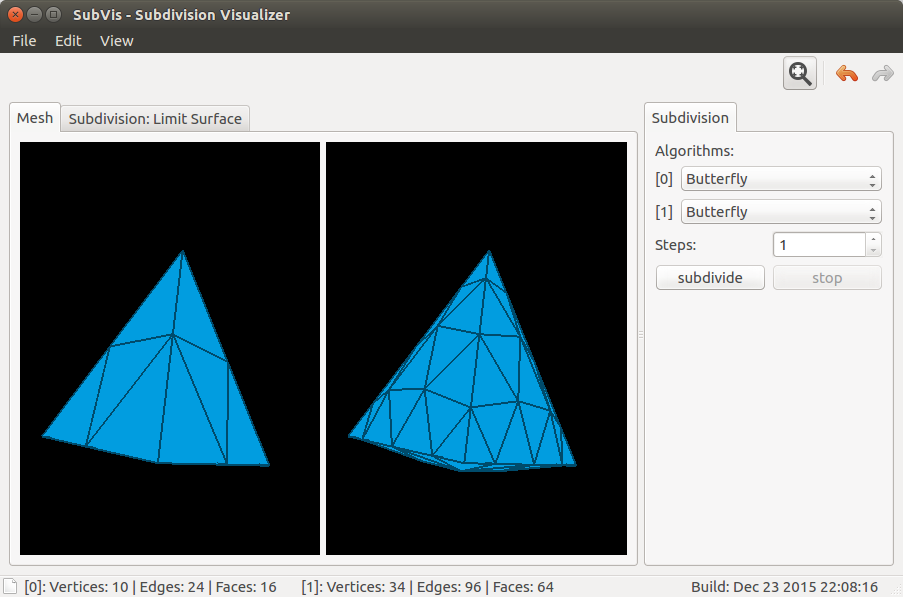
\includegraphics[width=0.7\textwidth]{content/media/sd_butterfly_screenshot.png}
  \caption{Subvis - Butterfly}
  \label{fig:sd_butterfly_screenshot}
\end{figure}

\subsection{Modified Butterfly}

Der Modified Butterfly ist nach \autoref{sec:modbutterfly} implementiert.
Die Klasse \emph{SdButterfly} erbt jedoch nicht von \emph{SdTriangle},
sondern direkt von \emph{SdButterfly}, da dieser bis auf Ausnahmeregeln
identisch mit dem Butterfly Algorithmus ist. In \emph{SdButterfly}
muss für eine korrekte Implementierung somit nur noch die Methode
\emph{compute\_edge\_point} überschrieben werden.
\autoref{fig:sd_modbutterfly_screenshot} zeigt einen Unterteilungsschritt.

\begin{figure}
  \centering
  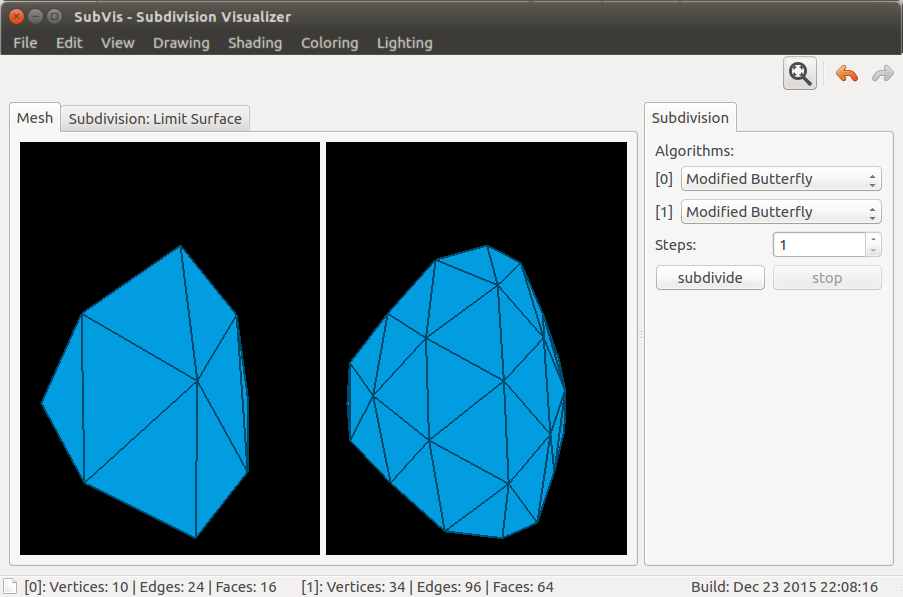
\includegraphics[width=0.7\textwidth]{content/media/sd_modbutterfly_screenshot.png}
  \caption{Subvis - Modified Butterfly}
  \label{fig:sd_modbutterfly_screenshot}
\end{figure}














